\documentclass[10pt,a4paper,danish]{article}
%% Indlæs ofte brugte pakker
\usepackage{amssymb}
\usepackage[danish]{babel}
\usepackage[utf8]{inputenc}
\usepackage{listings}
\usepackage{fancyhdr}
\usepackage{hyperref}
\usepackage{booktabs}
\usepackage{graphicx}
\pagestyle{fancy}
\fancyhead{}
\fancyfoot{}
\rhead{\today}
\rfoot{\thepage}

% Opsæt indlæsning af filer
\lstset{
  language=Python,
  extendedchars=\true,
  inputencoding=utf8,
  linewidth=\textwidth, basicstyle=\small,
  numbers=left, numberstyle=\footnotesize,
  tabsize=2, showstringspaces=false,
  breaklines=true, breakatwhitespace=false,
}

%% Titel og forfatter
\title{Informationsteknologi: Projekt e-læring \\ Projektkursus: Systemudvikling \\Forår 2011}
\author{Arinbjørn Brandsson (hkt789)\\Lasse Ahlbech Madsen (xsc606)\\Naja Mottelson (vsj465)\\Søren Pilgård (vpb984)\\
\\
Gruppeid : LO6\\
\\Instruktor: Lasse Nørregaard}

%% Start dokumentet
\begin{document}

%% Vis titel
\maketitle
\newpage

%% Vis indholdsfortegnelse
\tableofcontents
\newpage

%% HER STARTER RAPPORTEN
\section{Formål}
\subsection{Systemdefinition}
Systemet består af et digitalt interaktivt læringsværktøj hvis mål er at indføre elever på gymnasiefaget Informationsteknologi i programmering af systemer i forskellig størrelse. Disse systemer vil primært være fokuseret på udvikling af spil, men bredt datalogisk kompetencegivende. Systemet opbygges som et hjælpeprogram, som kører ved siden af brugerens teksteditor og en række præetablerede programmeringsforløb som eleven kan deltage i. Et forløb består af en række trin - konkrete programmeringsopgaver som hver indeholder en beskrivelse, en række hints samt et sæt tests der holder styr på om brugeren har opfyldt målet for hvert trin. Når brugeren har gennemgået alle trinene vil vedkommende have et komplet spil der kan afvikles seperat fra Udviklingsværktøjet. Systemet vil blive udviklet som en skrivebordsapplikation der kan afvikles lokalt på den enkelte brugers datamat/foldedatamat eller på datamater i gymnasiets eventuelle it-rum.

\subsection{BATOFF}
\begin{itemize}
\item \textbf{Betingelser}: Gymnasieelever med begrænsede programmering- og systemudviklingserfaringer. 
\item \textbf{Anvendelsesområde}: Eleven som bruger af systemet. Hvis værktøjet instaleres centralt på et
gymnasiums datamater vil der typisk være en Itadministrator hvis rolle er at opsætte systemet.
\item \textbf{Teknologi}: Systemet designes til at kunne køre på almindelige hjemmedatamater/foldedatamater.
Systemet vil blive baseret på python samt forskellige biblioteker dertil (i særdeleshed biblioteket pygame)
\item \textbf{Objekter}: En bruger som udvikler et spil i forbindelse med et forløb af opgaver. 
\item \textbf{Funktion}: Udvikling af spil.
\item \textbf{Filosofi}:  Digitalt interaktivt læringsværktøj
\end{itemize}

\section{Problemområde}
Eftersom vores system ikke gør brug af klynger til at gruppere klasser (vi har ingen klasser som er tilpas relaterede til at gøre dette brugbart) vil dette punkt stå tomt. 

\subsection{Struktur}
\begin{figure}[htb]
\begin{center}
\leavevmode
\includegraphics[scale=0.70]{klassediagram.png}
\end{center}
\caption{Klassediagram}
\label{fig:klassediagram}
\end{figure}

Strukturen for vores projekt (illustreret i figur \ref{fig:klassediagram}) blev relativt simpel: ”Bruger” klassen bestemmer hvilken opgaver man har og har ikke lavet, hvor klassen ”Opgaver” bestemmer forløbet. Vi bestemte at generalisere ”Færdig” samt ”Ikke Færdig/Fejl” under klassen ”Spil”, hvilket giver brugeren lov til at fortsætte til den næste opgave, eller fortæller at de skal fortsætte med opgaven. Det som skal noteres er at de to associeringer under ”Spil” også kan aggregere ”Opgaver” og ”Forløb” hvis den ene eller andens betingelser er mødt.

\subsection{Adfærdsmønster}
Hvad der vises i Figur \ref{fig:adfaerdsmoenster} er faktisk adfærdsmønstret for hele programmet - ikke udelukkende bruger-klassen. Som det bemærkes har vi bevæget os en smule væk fra bogens notation, eftersom dette forekom som en mere intuitiv beskrivelse af vores program. 
\begin{figure}[htb]
\begin{center}
\leavevmode
\includegraphics[scale=0.70]{adfaerdsmoenster.png}
\end{center}
\caption{Adfærdsmønster}
\label{fig:adfaerdsmoenster}
\end{figure}

\subsection{Hændelsestabel}
Se Figur \ref{fig:haendelsestabel} for en afbilding af vore hændelsestabel.
\begin{figure}[htb]
\begin{center}
\leavevmode
\includegraphics[scale=0.65]{haendelsestabel.png}
\end{center}
\caption{Hændelsestabel}
\label{fig:haendelsestabel}
\end{figure}

\section{Anvendelsesområde}

\subsection{(a) Brug}
\paragraph{}
Ved typisk brug af vores applikation vil man kunne finde 3 aktører: eleven, læreren og skolens systemadministrator.
Eleven vil stå for selve brugen af systemet og er langt den vigtigste aktør.
De to andre aktørers roller består i at få eleven til at benytte sig af systemet.
Deres rolle vil derfor være mere perifær og ikke specielt vigtig i udførslen af programmet.

\begin{table}[h]
  \begin{center}
    \begin{tabular}{r l l l}
      \toprule
      & Elev   & Lærer   & Administrator\\
      \midrule
      Installering    & (x)    &         & x\\
      Valg af forløb  & x      & x       &  \\
      Brug af program & x      &         &  \\
      Evaluering      &        & x       &  \\
      \bottomrule
    \end{tabular}
    \caption{Brugsmønster}
    \label{tab:brugsmoenster}
  \end{center}
\end{table}

I tabel \ref{tab:brugsmoenster} ses de 3 aktører og deres brugsmønstre.
Det ses hvordan brugen af programmet ligger hos eleven hvorimod det er lærerens opgave at evaluere om eleven har fået det ud af forløbet han skulle.
Dette er en typisk situation hvor en elev udfører en opgave og læreren giver en karakter. Installationen af programmet afhænger af gymnasiets organisation. Typisk vil det være en system administrator der varetager denne opgave. Hvis programmet installeres lokalt på elevernes egne datamater vil de dog som oftest selv stå for denne process.
Man kan forestille sig at læreren vælger at vælge hvilket forløb eleverne skal gennemføre men det kan også tænkes at læreren lader det være op til eleven selv at bestemme ud fra sit niveau. Det kan også være at læreren lader eleven fortsætte med andre forløb efter de har gennemgået et obligatorisk.
\\

Da vores program er forholdsvist letvægt og vi ikke har brug for at arbejde med hverken læreren eller administratoren er disses brugsmønstre af programmet indirekte, og ikke specielt relevante for den videre udvikling. Det kan dog være brugbar information i udbredelsen af programmet til gymnasier landet over.

\subsection{(b) Funktioner}
Hovedfunktionaliteten i programmet består i at kunne oprette eller indlæse et forløb. Samt at bevæge sig igennem forløbet trin for trin.
Når man starter programmet har man mulighed for enten at oprette et nyt forløb eller indlæse et allerede igangværende forløb.\\

Ved oprettelse af et nyt forløb vil man blive bedt om at indtaste sit navn samt vælge hvor på datamaten man ønsker at gemme sine ting. Derudover vælger man et af flere forskellige forløb hvorefter man kan gå igang. Til de forskellige forløb vil der være en kort beskrivelse der forklarer hvad forløbet går ud på, hvad man lærer af det, hvilke kvalifikationer man skal have for at gennemføre samt hvor svært det er.\\

Der bør her også være en hjælpe funktion der forklarer hvordan programmet virker og skal bruges (f.eks. at man skal bruge sin egen editor sideløbende). Denne hjælpe funktion bør automatisk starte første gang programmet startes, da det højst sandsynligt er her man har brug for hjælp.\\

Når man starter et nyt forløb bliver der udpakket en række kildekodefiler samt andre spilrelaterede filer i en mappe på det sted brugeren valgte at gemme. Her gemmes også en central fil der holder styr på hvilken bruger der ejer dette forløb samt hvor langt denne er nået. Denne udpakning er en engangsproccess der har til formål at forberede forløbet til brugeren.\\

Når man har åbnet et forløb kommer et nyt vindue op. Dette vindue udgør hoveddelen af programmet og det er herigennem selve forløbet gennemføres. Programmet er designet til at virke sideløbende med brugerens editor.\\

Da brugeren skal bruge sin egen editor til at tilgå og ændre filerne oprettet tidligere, vil det være en fordel hvis applikationen er placeret på skærmen på en sådan måde at brugeren kan se begge programmer på samme tid.
Da mange datamater i dag er widescreen\footnote{Se \url{http://store.steampowered.com/hwsurvey} under \textit{Primary Display Resolution}}
giver det mening at programmet er højere end det er bredt så det kan placeres til højre eller venstre for editoren så udnyttelsen af skærmpladsen optimeres.

Applikations vinduet er der hvor man inteagerre med forløbet.
Der vises her et trin ad gangen hvor kan finde en beskrivelse af opgaven samt hints. Her kan også være henvisninger til dokumentationen osv.

Applikations vinduet har 4 hovedfunktioner:
\begin{itemize}
  \item En \textit{kør} knap der starter spillet.
  \item En \textit{tilbage} knap der tilader brugeren at bladre tilbage gennem de allerede gennemførte trin for at kunne genlæse dem. 
  \item En \textit{frem} knap der kører alle tests op til næste trin. Hvis testsne lykkedes bladrer applikationen frem. Hvis en af testsne fejler hopper applikationen hen til det trin der fejlede.
  \item En liste over trin så brugeren kan hoppe mere end et trin frem/tilbage af gangen.
\end{itemize}
 
Testsne er en vigtig del af programmets funktionalitet.
For at se om brugeren rent faktisk har løst de opgaver der stilles i hvert trin, er der på forhånd sat en række unittests op til hvert trin. Disse tests skal være så uddybende at vi ved at hvis de gennemføres succesfuldt har brugeren gjordt det han skulle og vi kan derfor gå videre. Hvis en test fejler kan programmet udskrive en kommentar/hint til hvad der gik galt. En test kunne f.eks. være om den funktion brugeren skulle lave overhovedet er oprettet. Derefter kan man teste om outputtet til et givent input er korrekt. 
\subsection{(c) Brugergrænseflade}
Det er væsentligt at komplexiteten i vores program bliver så lille som mulig.
Der vil være nok udfordringer for brugeren når de skal i gang med at kode spillet i flere forskellige filer, samtidigt med at de skal have styr på deres editor.
Derfor skal programmet tilstræbe sig en så simpel brugergrænseflade som muligt.
Dette er heldigvis en overkommelig opgave da den primære funktionalitet i programmet består i at præsentere hvert trin samt køre tests af brugerens kode.

\paragraph{}
Vi kan derfor dele vores program ind i 3 hoved vinduer:

\paragraph{}
Det første vindue (kaldet startup) vil stille brugeren overfor et valg.
Vil du starte et nyt forløb eller vil du fortsætte på et gammelt?.
Hvis brugeren vælger at fortsætte på et tidligere startet forløb, vil en dialogboks komme frem hvori han kan navigere hen til forløbet og fortsætte på det.
Hvis brugeren derimod vælger at starte et nyt forløb bliver han dirregeret til hovedevindue nummer 2
Vinduet består af 3 knapper for at holde tingene så simple så mulige.
\begin{itemize}
\item \textit{Start nyt forløb} knappen
\item \textit{Fortsæt tidlligere forløb} knappen
\item \textit{Hjælp} knappen der åbner en dialogboks hvor man kan læse om brugen af programmet.
\end{itemize}

\paragraph{}
Det andet vindue (kaldet initialisation) vil være der hvor brugern kan starte et nyt forløb. Her skal han indtaste sit navn samt hvor på datamaten han ønsker at gemme sit projekt.
Det vigtiste valg ligger dog i at han skal finde ud af hvilket forløb han vil gå igang med. De forskellige forløb vil præsentere hvilket spil de laver, hvad man lærer af at lave dette spil samt hvor svært/hvilke krav der til brugeren før han kan gå igang (f.eks. at brugeren har styr på de grundlæggende dele af python)
Når brugeren er klar kan han trykke start.
Det er tænkt at dette vindue er delt op i tre dele, øverst er der et område med et tekstinput felt til brugerens navn, ved siden af det en knap der åbner en filbrowser op hvor brugeren kan vælge hvor han vil gemme, yderst til ventstre vil der sidde en hjælp knap med samme funktionalitet som i vindue 1.
Under den øverste bjælke vil vinduet være delt op i to områder, i venstre delen vil man se en liste af de forskellige forløb. Ved at klikke på et af forløbene vil man vælge det og i højre siden vil beskrivelsen nu komme frem. Nederst i det højre hjørne under beskrivelsen af det valgte forløb findes start knappen.
Start knappen vil kun komme frem såfremt et forløb er valgt, dette indikere overfor brugeren at det er det konkrete forløb der startes samt at det ikke giver mening at starte uden et forløb. Hvis ikke et navn er blevet indtastet vil startknappen være grå og uden mulighed for at blive trykket på.

\paragraph{}
Det tredje vindue er selve applikationen.
Vinduet er tænkt at fylde i højden men ikke i bredden.
Her vil man have en række knapper til at navigere med, samt et større område med tekst.
Øverst vil der sidde 4 knapper
\begin{itemize}
  \item En tilbage knap, symboliseret med en pil der peger mod venstre.
  \item En kør knap der starter spillet.
  \item En hjælp knap med et spørgsmålstegn der åbner hjælpesiden som i vindue 1.
  \item En frem knap symboliseret med en pil mod højre.
\end{itemize}


\subsection{(d) Den tekniske platform}
Teknisk består løsningen af 4 lag som set i figur \ref{fig:tekniskeplatform}
\begin{figure}[h]
  \begin{center}
    \includegraphics[scale=0.5]{afl2_teknisk_platform.png}
    \caption{Den tekniske platform}
    \label{fig:tekniskeplatform}
  \end{center}
\end{figure}

Nederst har vi Python laget. Python vil være den bærende del da både selve applikationen og spillet vil være udviklet i python.\\

Oven på python ligger Pygame. Pygame er et bibliotek til python bygget omkring SDL.
SDL (Simple Directmedia Layer) er et c-bibliotek der kan tage sig af 2d grafik, lyd, tastaturinput samt flere andre ting. SDL bliver brugt i en del spil\footnote{\url{http://en.wikipedia.org/wiki/List_of_games_using_SDL}}.
Pygame er bygget oven på SDL og giver tilgang til dets funktionalitet. Dette gør at man kan lave spil i python der kører forholdsvist hurtigt såfremt man benytter sig af de indbyggede metoder som er implementeret i C.\\

Oven på pygame laget ligger vores spilskelet. Det er den ufærdige kildekode til spillet som brugeren for udleveret og skal bygge videre på.
Dette lag skal hjælpe brugeren så han ikke skal bygge det hele fra bunden og så forløbet kan fokusere på de sjovere og mere relevante dele.\\

Øverst har vi et todelt lag bestående af vores applikation samt brugerens editor.
Det vil være gennem dette lag at brugeren inteagerer med de dybere lag.
Da formålet med projektet er at lære brugeren at udvikle, bør lagene være så transperante som muligt så brugeren kan forstå hvordan tingene hænger sammen. Samtidigt skal det dog laves på en sådan måde at brugeren ikke føler det kommer i vejen



\section{Anbefalinger}
\subsection{Nytte}
Projektet vil være nyttigt som en let og engagerende start på at lære et nyt programmeringssprog. I forhold til andre måde at tillære et nyt sprog på, er vores værktøj godt til gymnasieelever. Vi springer over de mindre interessante ting ved at lære et nyt sprog, og kaster dem direkte ud i det. Ifølge vores kunde er det største problem i forbindelse med undervisningen, at holde elevernes opmærksomhed. Hans erfaring er til gengæld at de f.eks. har været meget engageret i undervisningen, når de har udviklet spil. 

Vores værktøj er derfor ideelt til undervisning af gymnasieelever. De skriver selv størstedelen af koden, og sidder i sidste ende med et spil, som de frit kan lave om på og introducere nye ting til. De kan også løbende køre spillet og afprøve de ting de har implementeret. Det at de studerende efter hvert endt forløb er i besiddelse af et færdigt produkt, som de selv har udviklet, tror vi også har en god effekt på deres videre engagement og lysten til at arbejde videre. Ved kun at give hints, og tvinge dem til at komme på egne løsninger, kan vi udvikle dem som programmører og få dem til at tænke på nye måder over programmeringsrelevante problemer.

\subsection{Realiserbarhed}
Vi mener at projektet er udmærket realiserbart. Selve værktøjet er meget simpelt, og vi kan selv tilføje så mange forløb, som vi har tid til og/eller synes passende. Udviklingen af forløbene er sandsynligvis den mest tidskrævende faktor i projektet, de er til gengæld også meget omfattende, og især at lave dækkende unit-tests kan blive tidskrævende. Hvis vi skal have et værktøj med et anseeligt antal forløb, kan det blive et meget stort og tidskrævende projekt. Selve GUI'en og det overordnede værktøj er meget simple, og skulle ikke være noget problem at lave.

\subsection{Udviklingsstrategi}
Som det også nævnes afsnittet om projektarbejdet (prioritering af arbejdsopgaver), bliver næste kommende store opgave at påbegynde implementeringen af vores progra. Som det allerførste planlægger vi selv at implementere det første undevisningsspil, som skal indgå i det første forløb i værktøjet, hvorefter prioriterer at lave den del af programmet, som skal køre sideløbende med brugerens editor. Når denne del er konstrueret kan vi implementere resten af forløbene og arbejde på implementeringen a brugergrænsefladen og startskærmen. Det gør vi for at vi kan have et fungerende værktøj, i tilfælde af at vi ikke formår at færdiggøre projektet inden kursets afslutning.

\subsection{Økonomi}
Der er ingen økonomiske henseender at tage højde for. Arbejdskraften er gratis og der kræves hverken nyt hardware eller ikke-gratis software til at benytte værktøjet.

\section{Kravsspecifikation}
\begin{enumerate}
\item Systemet skal opbevare oplysninger om brugeren (navn, sti i filsystemet) og om deres rolle ift. programmet (bruger, lærer, systemadministrator)
\item Systemet skal kunne oprette nye forløb, samt tilgå gamle, ikke-gennemførte forløb lagret lokalt på brugerens datamat. 
\item Systemet skal indeholde funktioner til at registrere om et forløb er gennemført af en bruger. 
\item Systemet skal indeholde flere forskellige læringsforløb som brugeren kan gå i gang med.  
\item Systemet skal ikke tilbyde en integreret teksteditor.
\item Systemet skal indeholde funktionalitet til at køre brugerens kode samt fremvise fejlbeskeder.
\item Systemet skal for hvert trin i en programmeringsopgave tilbyde en tekst med hints og links til relevant dokumentation.
\item Brugergrænsefladen skal ligne (om end ikke være 100 procent ens med) figurerne (henvisning til figurerne)
\item Systemet skal være intuitivt at arbejde med - kun det programmeringsfaglige skal være krævende. 
\item Systemet skal kunne køre på både Windows, Mac og Linux
\item Systemet skal ikke stille hardware-krav som ikke mødes af størstedelen af almindelige hjemme-PC'er.
\end{enumerate} 

\section{Projektarbejdet}
Siden Delrapport 1 er der i særdeleshed en hændelse der har påvirket vores gruppearbejde, navnligt at et af vores gruppemedlemmer (Simon Maibom) har besluttet at falde fra faget og således ikke længere er en del af gruppearbejdet. Som også nævnt andetsteds i rapporten har dette bl.a. betydet at vi har måttet reducere opgavens omfang en lille smule for at tage forbehold for de færre mandetimer vi har at arbejde med. 
\newline
\newline
\subsection{Organisation af gruppen}
Som projektarbejdet skrider frem har vi opdaget en række uforudsete faldgruber ved den måde vi har organiseret gruppen internt. Som nævnt i Delrapport 1 valgte vi at have en meget veldefineret opdeling af projektledelse og projektarbejde, og at delegere ledelsesansvaret til et enkelt gruppemedlem. Skønt der er fordele ved denne måde at arbejde på (overskuelighed i uddelegering, undgåelse af store mængder spiltid ved bureaukratisk diskussion) kan vi konstatere, at det har resulteret i en uheldig forskel på hvor meget ejerskab det enkelte gruppemedlem føler overfor opgaven. Dette er et dilemma: Pointen i at lade ét menneske stå for den generelle organisering af gruppen er jo netop at fratage gruppen som helhed noget ansvar, men dette lader til at fratage den enkelte motivation til at deltage aktivt og til at opsøge andre opgaver end dem de får udstukket. I tillæg gør det gruppen ganske sårbar i tilfælde hvor den organisationsansvarlige af den ene eller anden årsag ikke kan udføre sine pligter optimalt, fx. sygdom eller pres fra deadlines i andre fag. 
\newline
\newline
Vores umiddelbare indtryk er at en del af denne problematik skyldes det stadium af designprocessen vi befinder os i. Som det står nu er hovedvægten af de opgaver vi udfører enten kollektive brainstorm/udviklingsopgaver/interviewopgaver, som er svære at uddelegere til enkeltpersoner. Vores antagelse er at opdelingen vil komme til sin ret organisatorisk når selve kodearbejdet kommer igang - indtil da har vi valgt at uddele et par af den organisationsansvarliges opgaver i gruppen for at sørge for en mere bred spredning af arbejdet. 
\newline
\newline
En anden problematik vi er løbet ind i er fordeling af arbejdsopgaver ved skrivning af rapporter. Som det er nu varierer gruppemedlemmernes erfaring og evne udi rapportskrivning en del, hvilket resulterer i at for meget af den endelige rapportskrivning ender med at blive udført af en eller to mennesker i gruppen. En del af denne problematik har sandsynligvis at gøre med at vi både ved sidste rapport og nuværende har ventet for længe med at uddele de konkrete arbejdsopgaver, så at de gruppemedlemmer der har besvær med rapportskrivning ikke har haft tilstrækkelig tid til at skrive de segmenter de er blevet gjort ansvarlige for. Ved Delrapport 3 regner vi derfor med at uddelegere de forskellige afsnit i rapporten på så tidligt et tidspunkt som muligt, så at de mindre erfarne gruppemedlemmer har bedre tid til at søge oplysninger og udbede sig hjælp til skrivearbejdet. 

\subsection{Kontakt med brugerne}
Siden Delrapport 1 har vi afholdt et enkelt yderligere møde med vores bruger, ved hvilket vi præsenterede den papir-mockup af systemet som beskrives og afbildes i afsnit 8. En udlægning af vores brugertesting er at finde i afsnit 9. 
\subsection{Dokumentationsstrategien}
Evalueringen af dokumentationsstrategien som efterfulgte Delrapport 1 har vist at vi overordnet set er ganske tilredse med den måde vi dokumenterer vores projekt. Sammenfattet gør vi dette ved at dokumentere interne koordinationsmøder i gruppen på 'traditionel' vis, at dokumentere møder med brugeren i stil med den aktion-reaktionsform der er beskrevet i teksten \emph{Back to thinking mode} (en tekst som også reviewes i denne rapport) samt at arbejde med checklister til brugermøderne som dokumenterer hvad vi håber at få ud af pågældende møde. 
\newline
\newline
Som nævnt i Delrapport 1 er ambitionen at lagre referater fra egne møder, referater fra møder med brugeren mm. i gruppens GitHub repository (vha. GitHubs indbyggede wiki-funktionalitet). Overførslen af data til GitHub er ikke dog endnu ikke blevet foretaget, af den simple grund at mailinglisten indtil videre fungerer udmærket som kombineret kommunikations- og lagringsmedium. En del af grunden til dette er sandsynligvis at vi endnu ikke har oplevet noget synderligt behov for at tilgå gammel dokumentation - når vi påbegynder implementering, samt ved fagets afslutning kan det antages at migreringen af materialer til et mere overskueligt medium bliver nødvendig.
\newline
\newline
Af problematikker og ting der kan gøres bedre i fremtiden har vi samlet følgende punkter: 
\newline
\newline
\begin{itemize}
\item Indholdet af referaterne fra gruppemøderne er indtil videre ikke særlig brugbart som andet end koordinationstekster. Som det er nu er en stor del af referatet udgjort af dokumentation af hvad status er på forskellige opgaver, samt hvem der skal have udført hvad inden næste møde. Dette er naturligvis nødvendig information, men det er ikke hvad man har brug for når dokumentationen skal læses igen om en måneds tid - da vil den vigtigste information sandsynligvis være hvilke overvejelser der ligger bag de valg vi træffer mht. design af programmet. Fremover vil vi derfor stræbe efter at dokumentere diskussionerne ved møderne i ligeså høj grad som de praktiske koordineringsbeslutinger. 
\item For at gøre dokumentationen af gruppemøderne så sammenhængende som muligt har vi fastsat én person med ansvar for referat, og lader ordstyreransvaret gå på omgang imellem de resterende gruppemedlemmer fra møde til møde. Dette er også for at sørge for at uddele den organisationsansvarliges opgaver en smule mere bredt udover gruppen. 
\item Det har været problematisk for os at skelne imellem hvilke møder der skal og ikke skal dokumenteres med referat. Når vi fx. afholder et kort møde med henblik på at fordele opgaver til skrivning af rapport virker det for arbejdskrævende at føre et fuldt referat. Under mødet kan der dog let opstå uplanlagte diskussioner af programmet som kan resultere i ændringer i design, og disse bør bestemt dokumenteres. Vores løsning har indtil videre været at affotografere tavlen brugt til at skitsere evt. ændringer og bruge disse billeder som dokumentation. Dette er dog ikke optimalt, da billeder kan være svære at afkode hvis man skal se tilbage på diskussionen på et senere tidspunkt. 
\end{itemize} 

\subsection{Mødeform}
Siden Delrapport 1 er vi gået ned til kun at mødes fast en gang om ugen. Dette er delvist fordi vi nu er færre mennesker i gruppen, og således kan håndtere flere af koordinationsspørgsmålene på en ad hoc-basis, men også fordi der generelt ikke lod til at være tilstrækkeligt med kollektive opgaver til at nødvendiggøre to møder. 

\subsection{Styring og prioritering af arbejdsopgaver}
Hidtil har vores hovedfokus i projektarbejdet været at definere rammerne for programmet, samt at forsøge at finde en overskuelig måde for os at samarbejde som gruppe. Det kan dog ikke nægtes at den konkrete kodeopgave vi har valgt varierer indholdsmæssigt fra de fleste projekter i PK-SU, og potentielt kan blive kompliceret at implementere. En af de vigtigste opgaver for os i den kommende tid vil derfor være at kode en fungerende prototype, som vi kan præsentere for kunden og brugergruppen. For at sørge for at komme godt i gang med kodeopgaven lægger vi ud med en 'kode-uge' i påske-ugen, hvor vi regner med at kode skelettet til det første prototypespil, samt de indledende ting ved selve applikationen. 

\section{Brugergrænseflade}
Se Figur \ref{fig:startvindue}, \ref{fig:hovedvindue} og  \ref{fig:nytforloeb} for en dokumentation af vores brugergrænseflade-mockup. 

\begin{figure}[h]
  \begin{center}
    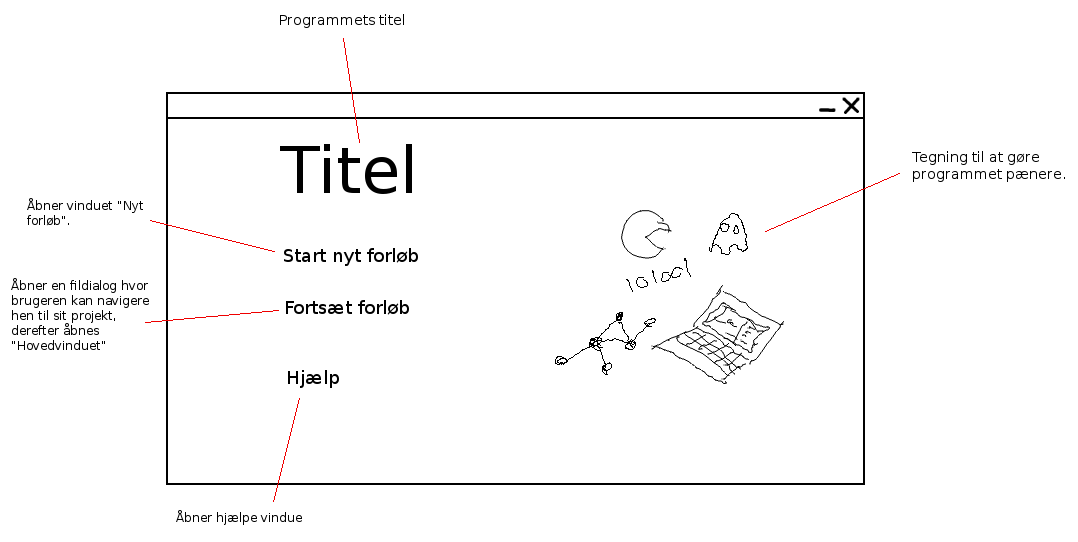
\includegraphics[scale=0.4]{startvindue.png}
    \caption{Programmets startvindue}
    \label{fig:startvindue}
  \end{center}
\end{figure}
\newpage

\begin{figure}[h]
  \begin{center}
    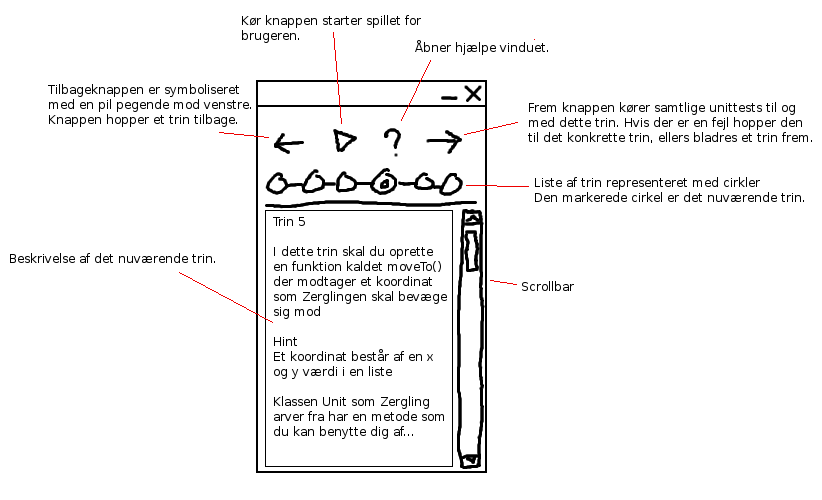
\includegraphics[scale=0.4]{hovedvindue.png}
    \caption{Programmets hovedvindue}
    \label{fig:hovedvindue}
  \end{center}
\end{figure}
\newpage

\begin{figure}[h]
  \begin{center}
    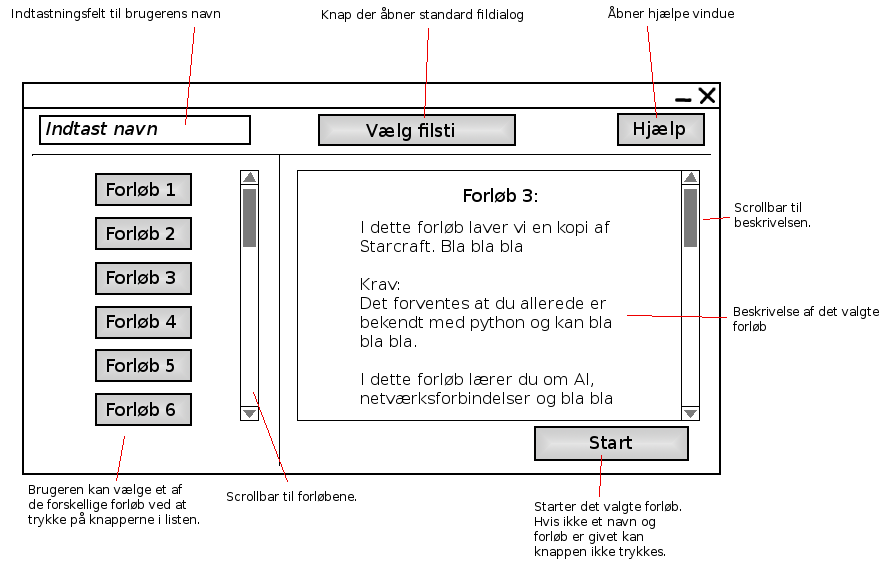
\includegraphics[scale=0.4]{nytforloeb.png}
    \caption{Et nyt forløb}
    \label{fig:nytforloeb}
  \end{center}
\end{figure}
\newpage


\section{Evaluering af brugergrænseflade}
Vi aflagde et besøg på Greve Gymnasium d. 4. april, hvor vi holdt et møde med kunden inddelt i to dele: Først et indlende møde med underviseren Bo Christiansen, hvor vi fortalte ham om udviklingen i projektet og modtog input på de valg vi har truffet hidtil. Dette blev efterfulgt af et møde med hans datalogiklasse i løbet af hvilket vi foretog den første brugerevaluering af vores grafiske grænseflade. Inden mødet med Bo Christiansen havde vi (som nævnt i vores dokumentationsstrategi) i gruppen diskuteret hvad vi gerne ville opnå med mødet - vi overvejede at formulere en tilsvarende for mødet med klassen, men kom frem til at det vigtigste ved brugertests netop er at undgå at komme med for mange præetablerede idéer.
\subsection{Beskrivelse af brugertests}
Til den datalogitime vi benyttede til vores tests dukkede 4 ud af 7 gymnasieelever op - i det følgende udgør disse fire elever vores testpersoner. Vi indledte vores brugertests med først at forklare testpersonerne lidt yderligere om hvad vores program går ud på (vi havde ikke forberedt en visuel præsentation til denne del af testen, men benyttede tavlen til at visualisere programmet), samt hvordan afprøvningen ville komme til at foregå. 
\newline
\newline
Til afprøvning har vi fremstillet en papir-mockup af vores programs grafiske brugergrænseflade (se figurer), som modellerer alle de forskellige menuer og vinduer der kan blive præsenteret for brugeren. Vi udførte afprøvningen ved at bede hver enkelt elev forestille sig at papirmodellerne havde samme funktionalitet som et fungerende program, og at interagere med dem som sådan ved at klikke på knapper o.lign. Ved hver afprøvning var så allokeret et gruppemedlem med en kopi af mock-uppen som kunne navigere testpersonen til den side/menu/scrollbar de på et givent tidspunkt havde forespurgt samt et gruppemedlem med ansvar for at notere brugerens reaktioner og input. Vi nåede desværre kun 3 afprøvninger, da datalogitimen sluttede inden vi var kommet igennem alle eleverne.
\subsection{Respons fra testpersonerne}
Vi ledte testpersonerne igennem 3 relaterede use-cases: At oprette et nyt forløb, at indlæse et gammelt forløb, og at arbejde på et igangværende forløb.
Responsen fra testpersonerne var generelt ganske positiv: Alle tre testpersoner havde forholdsvis nemt ved at forstå hvordan man navigerede rundt i grænsefladen, skønt det trak den samlede oplevelse ned at de ikke kunne prøve programmet 'sammen med' en teksteditor. Umiddelbart var det forløb der skabte de fleste problemer at oprette nye forløb - de fleste af gymnasieeleverne lod ikke til øjeblikkeligt at forstå hvad der ville ske når man klikkede på ikonerne i programmets startmenu. En del af dette kan muligvis have at gøre med at de stadig var i gang med at stifte bekendtskab med vores mockup, men ved næste design-gennemgang vil vi tage layoutet af startmenuen op til diskussion. 

Den generelle respons vi fik på layoutet af det vindue hvori brugeren kan køre koden (figur) tydede ligeledes på at en revision kunne overvejes; skønt størstedelen af testpersonerne havde nemt ved at forstå selve funktionaliteten (frem- og tilbageknapperne, kør-knappen, fejlmeddelelsessektionen) var der flere der kommenterede at selve vinduet virkede uoverskueligt ved første øjekast, samt at teksten måske burde reduceres eller gøres mulig at folde sammen. 


\section{Resuméer}
\subsection{Andersen, N. E. et al. (1986): \emph{Professionel Systemudvikling}}
Uddraget fra Andersens \emph{Professionel Systemudvikling} argumenterer for at når en projektgruppe starter et
nyt projekt, vil deres tid i begyndelsen være bedst brugt på at lave en projektetablering, og at de få dage
som er brugt på projektmøder og forberedelse til disse møder er godt brugt.
Artiklen forklarer at projekter skal etableres for at projektet kan gøre fremskridt. Et projekt skal etableres
da dette
\begin{enumerate}
\item Bidrager til at gøre udgangspunktet realistisk
\item Øger projektgruppens forståelse og accept af udgangspunktet for forløbet
\item Kan klarlægge og påvirke forholdet mellem projektgruppen og omgivelserne
\item Styrker gruppen, og
\item Giver holdepunkter til styringen af projektets videre forløb.
\end{enumerate}
Dog erkender uddraget at projektetablerings-processen kan have nogle ulemper, så som at gruppen skal have tid til at holde nogle gruppemøder tidligt i processen, hvori alle deltagerne skal bruge kræfter på at udarbejde projektgrundlag, samt diskussion og forhandlinger med andre grupper og enkeltepersoner. Og disse omkostninger bliver kun større jo flere deltagere der er, og jo større projektet er. Men uddraget følte at disse omkostninger er nødvendige, da i fremtiden, gruppen vil spare tid og energi ved at holde en projektetablering.

Uddraget fortæller også at projektetableringsprocessen har to formål: At etablere selve projektet,  samt at få projektgruppen til at blive et fagligt og socialt velfungerende arbejdsenhed. Uden et projektetablering vil de individuelle deltagere forblive koncentreret om deres individuelle opgaver, hvilket betyder at de ikke ved meget om de grundlæggende idéer om gruppen, da deres opgaver er baseret på den oprindelige beskrivelse af opgaven. Ved at holde en projektetablering vil alle deltagerne have en større forståelse for projektet, hvilket gør arbejdspladsen til en mere velfungerende fagligt arbejdsenhed. Og under projektetableringen, så hvis alle deltagerne fortæller om hvad de forventer fra projektet fagligt, uddanelsesmæssigt, karrieremæssigt og personligt. Ved at lade deltagerne gøre dette vil chancen for at deltagerne kæmpes indbyrdes for magt over projektet minimeres, da alle ved hvad de andre forventer fra projektet, hvilket gør arbejdspladsen socialt velfungerende.

Det betaler sig også at lave et projektgrundlag, da dette lader gruppen sammenligne projektets hidtil forløb, og projektgrundlagets, hvilket giver gruppen motivering for at fortsætte, samt det også lader deltagerne se hvordan projektet udvikler sig.

Men vigtigst, ifølge uddraget, er at forhindringerne gør behovet for projektetablering større, når deltagere falder fra, eller når nye deltagere kommer frem. Projektetableringen hjalp os da vi var 5, da det hjalp os med at finde ud af hvordan vi skulle tackle at vi havde så mange for vores projekt, og det hjalp os da en af vores gruppemedlemmer faldt fra. For da det skete, blev vi nødt til at genoverveje hvad vi ville med projektet, da vi nu ikke ville kunne gøre de ting som vi originalt havde planlagt for projektet. Der hjalp projektetableringen, for ved at læse det igennem kunne vi se at nogle 'positive' ting ved at deltagerne faldt fra (fx. ville kommunikation internt blive nemmere), og med projektetableringen kunne vi genorverveje vores rammer for projektet, og lave (lidt) om på projektet for at redegøre for vores lidt mindre gruppe. Og med projektetableringen blev vi enige om hvordan vi skulle dokumentere vores korrespondence med vores kilent, hvilket hjalp efter vi havde haft nogle møder med vores klient.

\subsection{Leif O. Jepsen, Lars Mathiassen og Peter A. Nielsen: \emph{Back to thinking mode: Diaries for the management of information systems development projects}}

Artiklen handler om effektivisering af informationsbehandling i en gruppe under et systemudviklingsprojekt. Den argumenterer specifikt for brug af dagbøger, som et redskab til at forbedre behandling af indtryk og erfaringer. Dagbogens styrker ligger i dens evne til at få en til at reflektere over projektet og dets gang. Forfatterne mener specifikt at dagbøger er gode til at skabe nye arbejdsrutiner og øge gruppens forståelse af deres egne brugsmetoder. Tanken er at man bruger dagbogen fremadrettet, og planlægger ud fra ens erfaringer, så man kan opnå bedre resulter. Den er selvfølgelig også nyttig når man skal evaluere et projekt. Dagbøger kræver en hvis disciplin at vedligeholde, men dette mener forfatterne også er en fordel, da det smitter af på projektet. Som argumentation for brugen af dagbøger sammenligner de dem med normale dagbøger, der ifølge Rainer (1983) er selvforbedrende. De hævder at den også kan bruges som en kollektiv refleksionsprovokatør og forårsage professionel forbedring. 

Tiden der skal sættes af til at holde en ordbog er dog betragtelig, og i korte forløb, hvor der allerede er en meget begrænset tid afsat til projektet. Artiklen stiller selv spørgsmålet, om teknikken er effektiv nok fra en cost/benefit betragtning, men besvarer det ikke. I et længere forløb med mere kundekontakt, kunne en dagbog givetvis være gavnlig, men i et projekt som vores, med sideløbende projekter og begrænset tid, må det betragtes som ekstra arbejde med for lille en gevinst.

En betydelig del af artiklen er også skænket til aktion-reaktions skemaer, til dokumentation af interviews og møder. De hjælper med at give overblik og forståelse for hvordan mødet egentlig forløb i forhold til blot at nedfælde, hvad der blev diskuteret og besluttet. Man kan se, hvor man er gået forkert af hinanden, og i fremtiden ændre og forbedre ens interview metoder. 

\subsection{Ehn, P. og Kyng, M.: \emph{Cardboard computers: Mocking it up or hands-on the future}}

Artiklen omhandler brugen af såkaldte mock-up modeller af ikke-færdiggjorte produkter. Ideen er at man laver en model af det ønskede produkt, og på den måde kan få bedre ideen om, hvorvidt designet f.eks. er brugervenligt og let at navigere, hvis vi snakker software. Det er især en god teknik overfor kunden, så man kan undersøge, hvorvidt det der virkede intuitivt for en selv, også er det for andre. En vigtig del af brugen af mock-up modeller er også, at kunden og producenten nemmere kan blive enige, om hvad det ønskede produkt er, og åbner op for en dialog, der ellers kan være svær at opnå, da de to grupper typisk befinder sig på to ret forskellige niveauer. 

Mock-up modeller har også ressourcemæssige fordele, da man ved at afprøve produktet med disse midler, bedre kan sikre så at det rent faktisk er en god løsning, der arbejdes hen imod, og man mindsker derfor risikoen for spild og evt. at stå med et færdigt produkt, som ikke var det kunden var ude efter. Det er dog ikke nødvendigvis nemt at fremstille modellerne. I forhold til de udgifter, der kan være i forbindelse med konstruktionen af det endelige produkt, er det dog som regel en god investering alligevel. De kan typisk fremstilles af billige materialer, så det største problem er typisk, at de kan være meget tidskrævende at fremstille, og det kan være et stort arbejde blot at lave en lille ændring af dem. 

Artiklen diskuterer desuden brugen af computerprototyper, hvor man ved hjælp af forskelligt software kan lave nogle relativt avancerede mock-ups. De har den styrke, at de virker mere ”rigtige”, til gengæld mister de noget af simpelheden, som papir modellerne er stærke i, og der kan være udgifter til indkøb af programmel. Forfatterne er desuden ikke sikre på, hvad der er ”sjovest”.

Som beskrevet i afsnit 9 afprøvede vi selv en papirprototype af vores produkt på vores kundes elever. Vi havde gode erfaringer med dette, selvom de ikke var særligt engageret, fik vi den opfattelse, at prototypen var nogenlunde intuitiv, og at vi kunne fortsætte arbejdet med vores foreløbige design for øje. Vi brugte dog en del tid på at fremstille disse, og det virkede en smule præmaturt så tidligt i udviklingsprocessen. En styrke vi oplevede ved papirsmodellen, var netop det, at alle kan se, at det bare er en model, og derfor ikke forholdte sig til dets egentlig kunnen, men blot til designet når vi diskuterede den.

\end{document}


